\section{Discussion}


\subsection{Latitude profiles}
\label{sec:Latitude_profiles}

We want to compare the results of our different models. In Figure \ref{fig:Profiles} we show the integrated flux in the energy range $10 - \SI{100}{GeV}$ as a function of latitude $b$. The regions have a width of $\ang{4}$ for $|b|<\ang{10}$ and $\ang{10}$ for $|b|>\ang{10}$ in latitude and a width of $\ang{10}$ in longitude, that is $\ang{0} - \ang{10}$ to the East of the GC an $\ang{-10} - \ang{0}$ to the West of the GC. The profiles of the three models show the residual including the FB, i.e. for the low-energy model this is the residual, for the rectangles model it is the sum of residual and rectangles template, and for the GALPROP model it is the sum of residual, FB template and GC excess template, as decsribed in section \ref{sec:Modeling}. For comparison we show the data with PS mask.\\
We observe an agreement between all models and a East-West assymmetry close to the GC. While for positive longitudes we find oversubtractions in some models, for negative longitudes there is an increase of flux in the Galactic plane by at least a factor of 2 for all models. The residual of the GALPROP model differs from the low-energy and rectangles model in the Galactic plane by a factor of $2-3$. This is a result of the large oversubtractions at low latitudes.
Also the data shows a slight East-West assymmetry in the flux around the GC.


\begin{figure*}[h]
    \begin{subfigure}{0.5\textwidth}
        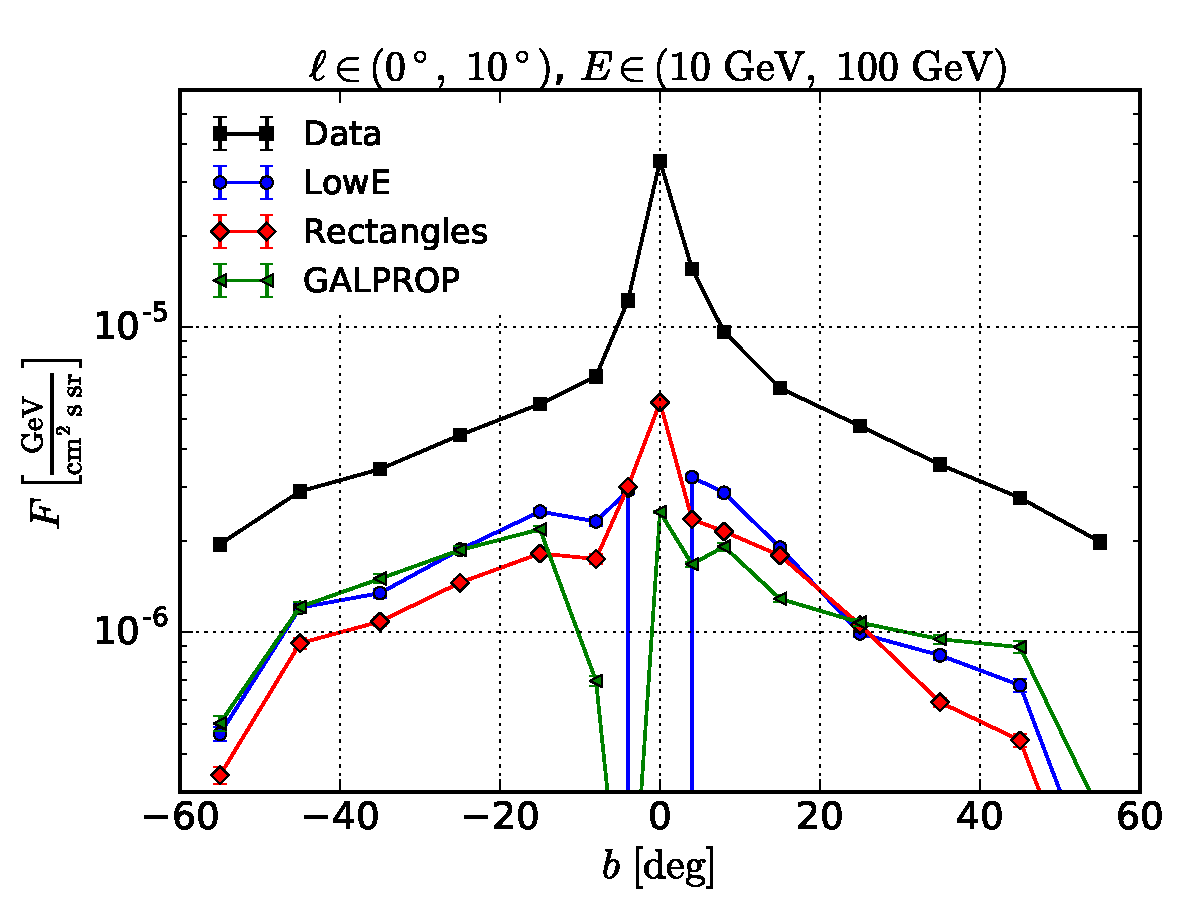
\includegraphics[width=\textwidth]{plots/Profiles_l=1_source_range_1.pdf}
    \end{subfigure} 
    \begin{subfigure}{0.5\textwidth}
        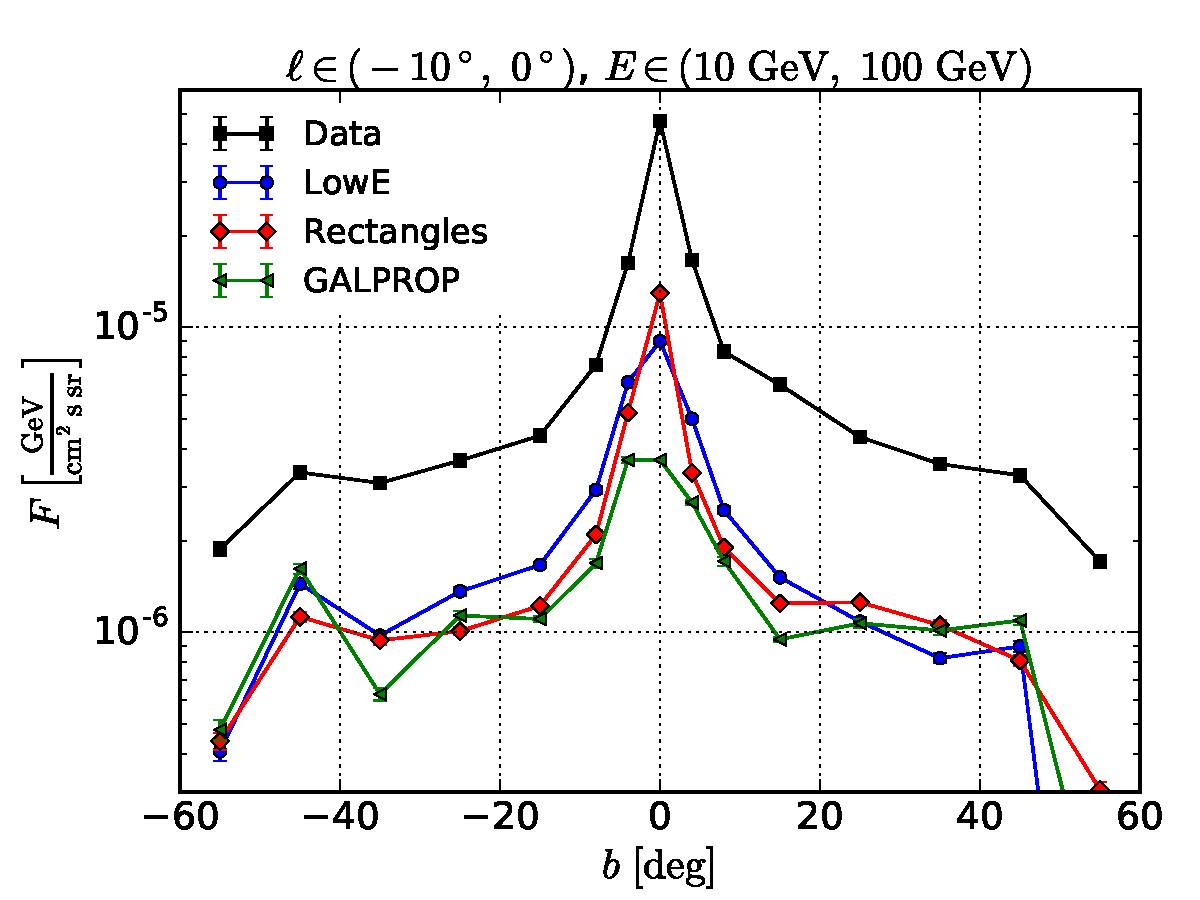
\includegraphics[width=\textwidth]{plots/Profiles_l=0_source_range_1.pdf}
    \end{subfigure}
    
  	\caption{Latitude profiles of the different model residals and the data with PS mask in integrated flux in $10 - \SI{100}{GeV}$. The width of the regions in longitude is $\ang{10}$, i.e. $\ang{0} - \ang{10}$ to the East of the GC (left) and $\ang{-10} - \ang{0}$ to the West of the GC (right).}
  	\label{fig:Profiles}
\end{figure*}

\subsection{Comparison of the spectra at different latitudes}

\begin{figure*}[h]
    \begin{subfigure}{0.5\textwidth}
        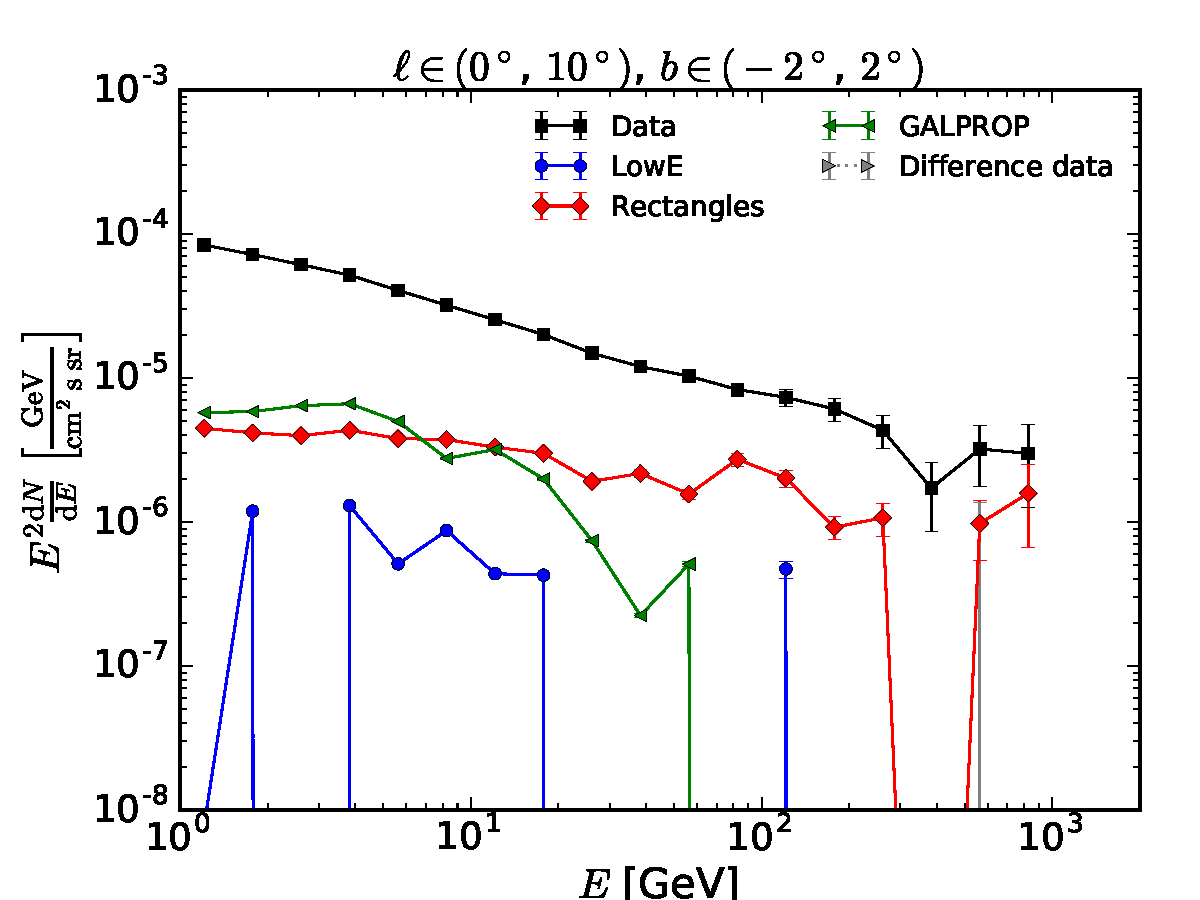
\includegraphics[width=\textwidth]{plots/SED_all_models_source_l=5_b=0.pdf}
    \end{subfigure} 
    \begin{subfigure}{0.5\textwidth}
        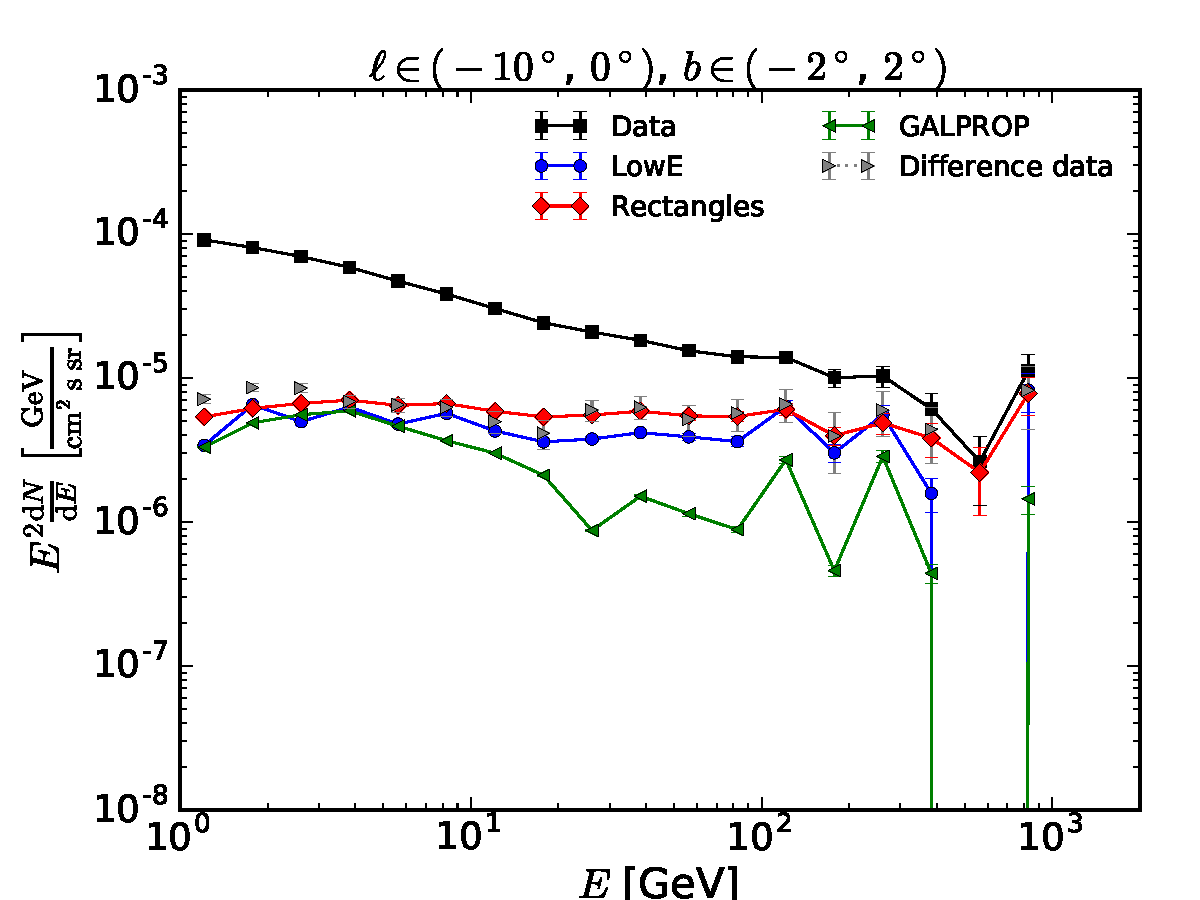
\includegraphics[width=\textwidth]{plots/SED_all_models_source_l=-5_b=0.pdf}
    \end{subfigure}
  	\caption{SED of the model residuals, the data with PS mask and the difference in the data with PS mask West minus East. The width of the regions in longitude is $\ang{10}$, i.e. $\ang{0} - \ang{10}$ to the East of the GC (left) and $\ang{-10} - \ang{0}$ to the West of the GC (right).}
  	\label{fig:SED_all}
\end{figure*}

In the following, we want to test the hypothesis of a harder energy spectrum inside the FB region in the Galactic plane. We first compare the spectral energy distribution (SED) of the different model residuals in Figure \ref{fig:SED_all}. The differential flux is averaged over regions to the East $(\ang{0} - \ang{10})$ and West $(\ang{-10} - \ang{0})$ of the GC, in a very thin stripe covering the Galactic plane $b \in (\ang{-2},\ \ang{2})$. For comparison we show the data with PS mask and the difference in the data West minus East, which is positive in every energy bin in the shown latitude band.

For negative longitudes, all models give similar results. We again observe that the differential flux of the GALPROP model is smaller than the differential flux of the other models, wich is consistent with the observation in section \ref{sec:Latitude_profiles}. We also find an assymmetry in the flux of the data with PS mask. The difference of the data West minus East is similar to the flux of the low-energy and rectangles model. The spectra at positive longitudes show large oversubtractions and an overall softer spectrum. %\Laura{Should we show here the plots for (-6,-2) and (2,6) deg latitude also?}
%\dima{I'm not sure, it will take space}

To compare the behavior of the energy spectra at high energies for different latitudes, 
we fit a log-parabola
 \be
 f(E) = N_0 \left(\frac{E}{\SI{1}{GeV}}\right)^{-\alpha - \beta \ln(E)}
 \ee
in each latitude stripe. The local ``index'' of the spectrum at energy $E$ is
 \be 
n \equiv \frac{\de \ln f}{\de \ln E} = -\alpha - 2 \beta \ln\left(\frac{E}{\SI{1}{GeV}}\right).
 \ee
In Figure \ref{fig:logpar_index} we compare this log-parabola index $n$ as a function of latitude at $E = \SI{500}{GeV}$. 
%\Laura{You called it bubble! ;)} \dima{bubble removed}
Shown is $(2 - n)$ which corresponds to the SED index.
For positive longitudes the index is relatively soft ($2-n > 2$) for most of the latitudes, 
except high latitudes where the gamma-ray statistics is small.
For negative longitudes the index near the GC is $\approx -2$, 
which is significantly harder than the index at higher latitudes.
%\Laura{Would you like the x-axis of the log-par plot to show n-2?}
%\dima{yes, I'd suggest to put (2 - n) on the y-axis}
\begin{figure*}[h!]
    \begin{subfigure}{0.5\textwidth}
        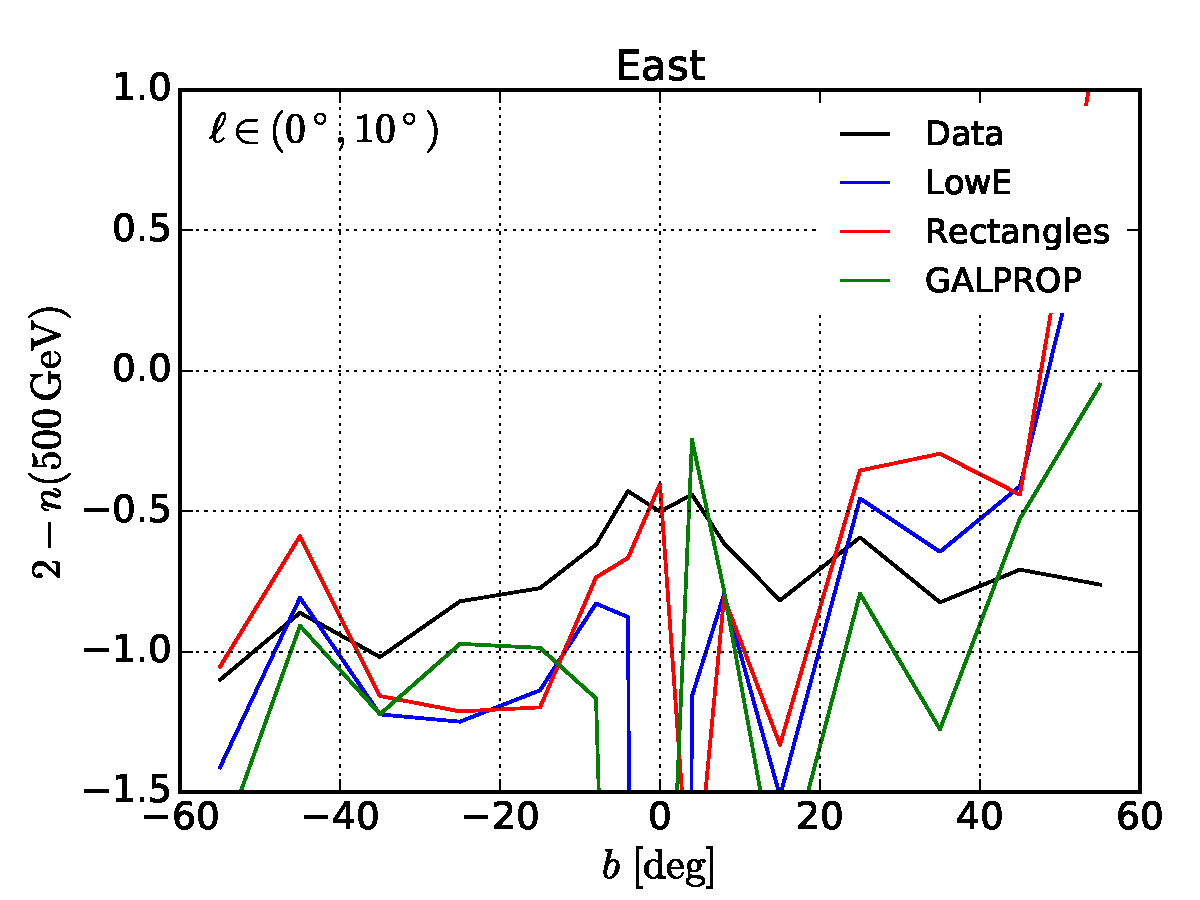
\includegraphics[width=\textwidth]{plots/LogParabola_n(500GeV)_l_in_(0,10).pdf}
    \end{subfigure} 
    \begin{subfigure}{0.5\textwidth}
        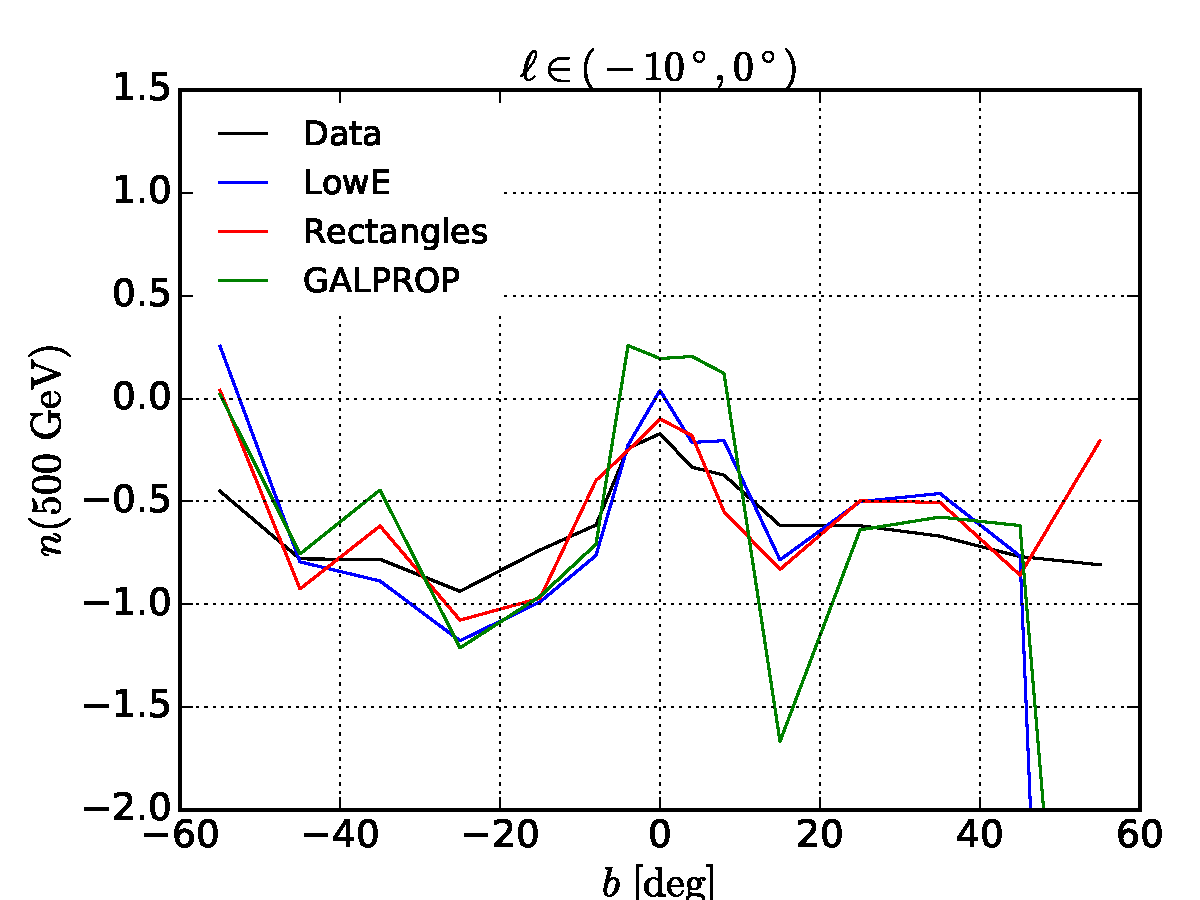
\includegraphics[width=\textwidth]{plots/LogParabola_n(500GeV)_l_in_(-10,0).pdf}
    \end{subfigure}
  	\caption{Index of the log-parabola (as defined in the text) at an energy $E\ = \SI{500}{GeV}$ as a function of latitude for the different model residuals. The width of the regions in longitude is $\ang{10}$, i.e. $\ang{0} - \ang{10}$ to the East of the GC (left) and $\ang{-10} - \ang{0}$ to the West of the GC (right).}
  	\label{fig:logpar_index}
\end{figure*}




\subsection{IC model of the gamma-ray emission}
\label{sec:IC_model}

Inverse-Compton (IC) radiation is produced in scattering processes of relativistic electrons on photons of the ISRF. The spectrum of the IC gamma radiation $(E \de n/ \de E)_{\gamma,\IC}\ [\SI{}{1/cm^3s}]$ depends on the density of ISRF photons $(\de n/ \de E)_\ISRF\ [\SI{}{1/GeVcm^3}]$ , the density of electrons $(\de n / \de E)_\el\ [\SI{}{1/GeVcm^3}]$ and the IC cross section $\sigma_\IC(E_\gamma, E_\ISRF, E_\el)$, taken from \citep{1970RvMP...42..237B}:
\be
\left(E\frac{\de n}{\de E}\right)_{\!\!\gamma,\IC}\! = c\int\!\! \int \left(\frac{\de n}{\de E}\right)_{\!\!\ISRF} \sigma_\IC\ \left(\frac{\de n}{\de E}\right)_{\!\!\el} \de E_\ISRF\, \de E_\el.
\label{eq:IC_spectrum}
\ee
The ISRF has three main components: starlight, IR and CMB. 
The IR and the starlight components are taken from the on-line distribution of GALPROP. 
For the CMB, we use the thermal spectrum with the temperature $\SI{2.73}{K}$.\\
We assume that the density of electrons as a function of energy follows  a simple powerlaw 
\be 
\left(\frac{\de n}{\de E}\right)_\el = n_\el \left(\frac{E_\el}{\SI{1}{GeV}}\right)^{-\gamma_\el} %\cdot \eto^\frac{E}{E_{\cut,\el}},
\label{eq:e_spectrum}
\ee
and determine the normalization $n_\el$ and spectral index $\gamma_\el$  by fitting the IC spectrum \eqref{eq:IC_spectrum} to the diffuse \Fermi data. For that, we determine the photon counts detected by \Fermi-LAT that correspond to the IC radiation generated by the electrons in the respective region. For a volume $V$ and a distance $R$ to the region, the detected counts per energy bin $E$ are 
\be
N_{\gamma,\IC}(E) = \left(E\frac{\de n}{\de E}\right)_{\!\!\gamma,\IC} \cdot V \frac{\tau(E_\gamma)}{4 \pi R^2} \cdot \de(\log E_\gamma),
\ee
where $ \de(\log E_\gamma)$ is the logarithmic size of the energy bin. Since the exposure $\tau(E_\gamma)$, which is averaged over the area on the sky, depends on energy, it can affect the shape of the electron spectrum. The quantities $V$ and $R$ only affect the normalization of the electron spectrum and will not be important until section \ref{sec:Interpretation}.\\
Now our model for the total detected counts is the sum of one of the foreground models and the counts generated by the electron density via IC scattering. As our baseline model for the foreground, we pick the rectangles model. We fit our model of the total counts to the actually observed total counts in that region (with PS mask) using Poisson likelihood and extract the parameters $n_\el$ and $\gamma_\el$ of the electron spectrum.\\

Figure \ref{fig:SED_with_fits} shows the residual of the rectangles model within the latitude stripes $b \in (\ang{2}, \ang{6})$, $b \in (-\ang{2}, \ang{2})$ and $b \in (-\ang{6}, -\ang{2})$ (as in Figure \ref{fig:SED_all}). The dotted line represents the best-fit IC spectrum for an electron distribution following a simple powerlaw.
%\Laura{Should we here compare with the spectral indices of the other models?} \dima{yes}
The spectral index to the West of the GC of the electron spectrum is relatively hard. For $b \in (\ang{2}, \ang{6})$ the spectral index varies between 2.92 and 3.15 for the three models, for $b \in (-\ang{2}, \ang{2})$ between 2.68 and 3.54 and for $b \in (-\ang{6}, -\ang{2})$ between 2.85 and 3.00. The softest spectrum in each latitude stripe is fitted to the GALPROP model. To the East of the GC the spectral indices vary between 2.97 and 5.09 in the three latitude stripes. 


We want to estimate the probability for the electron spectrum to have an exponential cutoff. For that we multiply an exponential cutoff $\exp(E_\el / E_{\el,\cut})$ to the electron spectrum \eqref{eq:e_spectrum} and determine the parameters analog to the procedure described before, using the rectangles model as the baseline foreground model.\\

%For the latitude stripe covering the Galactic plane, $b \in (-\ang{2}, \ang{2})$, adding a cutoff to the powerlaw does not improve the $\chi^2$-value both at negative ($\chi^2 \approx 135$) and positive longitudes ($\chi^2 \approx 128$).

%We determine the lower bound for the cutoff energy at a $\SI{95}{\percent}$-confidence level for our baseline model, the value in parenthesis gives the lowest value for all models: For negative longitudes we find a lower bound for the cutoff energy at $\SI{13.3}{TeV}$ ($\SI{2.9}{TeV}$), for positive longitudes at $\SI{491}{GeV}$ ($\SI{16}{GeV}$).

%Slightly below the Galactic plane, $b \in (-\ang{6}, -\ang{2})$, the $\chi^2$-value does not improve by exchanging the simple powerlaw by a powerlaw with a cutoff at negative longitudes ($\chi^2 \approx 76$). At positive longitudes the $\chi^2$-value improves slightly by adding the cutoff ($\chi^2 = 98$ to $\chi^2 = 87$). For negative longitudes we find a lower bound for the cutoff energy at $\SI{6.89}{TeV}$ ($\SI{6.89}{TeV}$), for positive longitudes at $\SI{818}{GeV}$ ($\SI{0.79}{GeV}$), at a $\SI{95}{\percent}$-confidence level.

\begin{figure*}[h!]
    \begin{subfigure}{0.49\textwidth}
        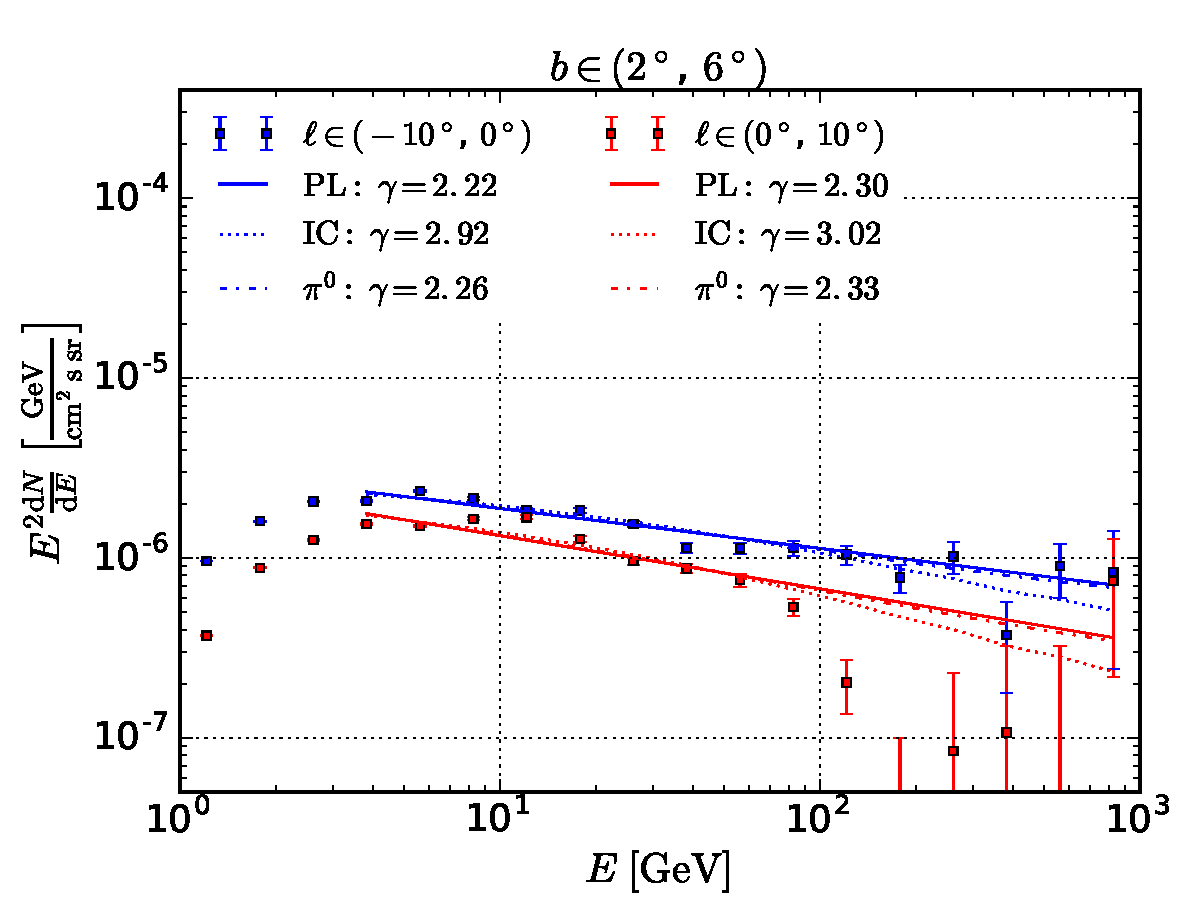
\includegraphics[width=\textwidth]{plots/SED_boxes_source_4.pdf}
    \end{subfigure}\\
    \begin{subfigure}{0.49\textwidth}
        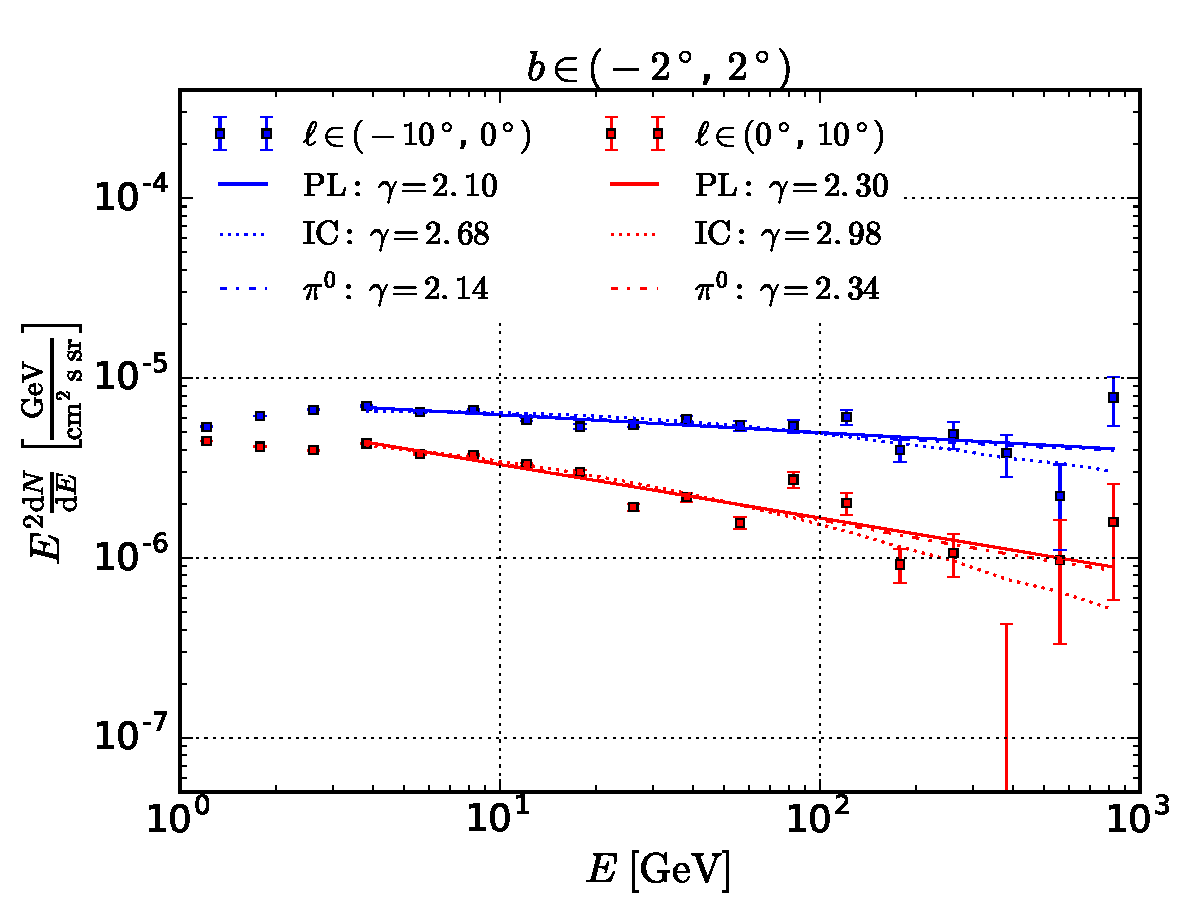
\includegraphics[width=\textwidth]{plots/SED_boxes_source_0.pdf}
    \end{subfigure} \\
    \begin{subfigure}{0.49\textwidth}
        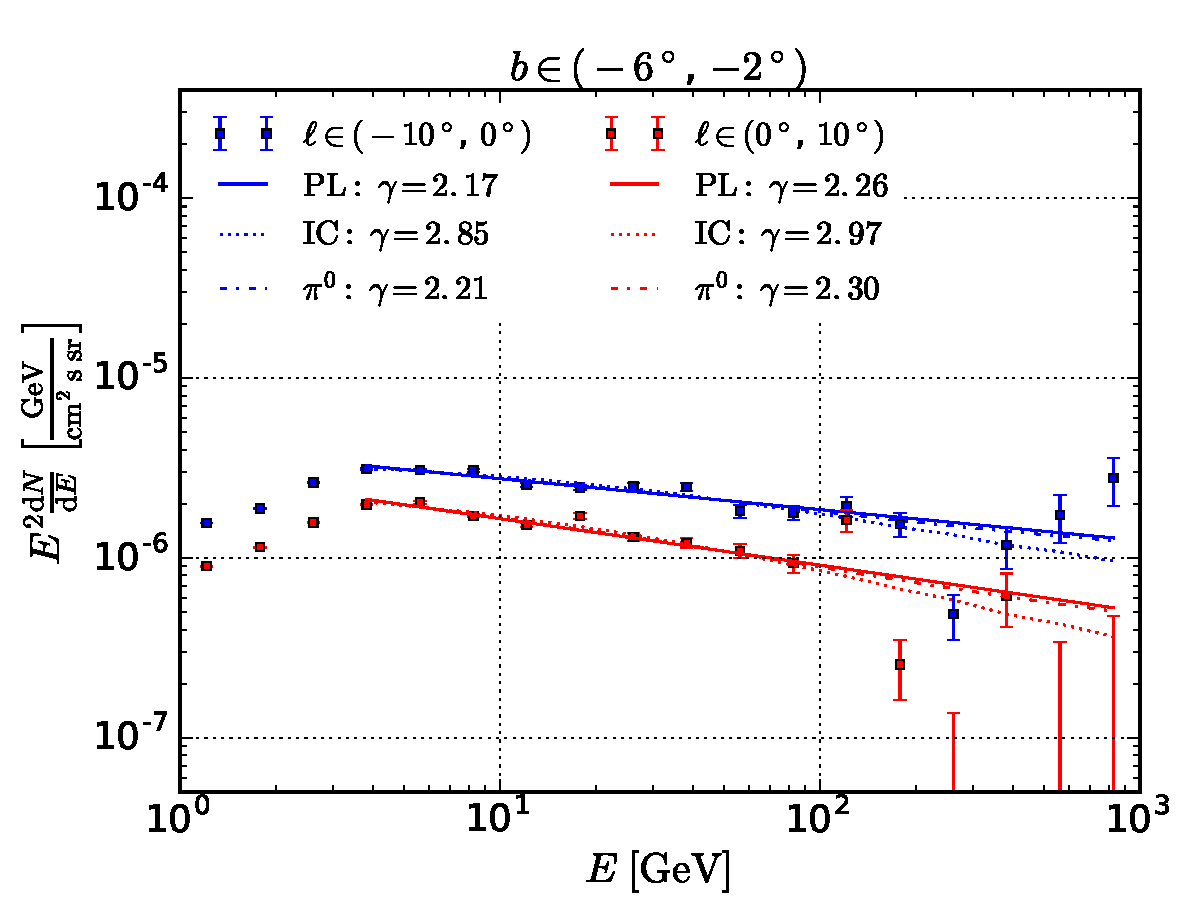
\includegraphics[width=\textwidth]{plots/SED_boxes_source_-4.pdf}
    \end{subfigure}
  	\caption{SED of rectangles-model residual in the latitude stripes $(\ang{2}, \ang{6})$, $(\ang{-2}, \ang{2})$ and $(\ang{-6}, \ang{-2})$ for negative (blue) and positive longitudes (red). We determine the spectral index of a powerlaw (PL), of an electron distribution emitting gamma-rays via IC and of a proton distribution emitting gamma-rays via $\pi^0$-decay.}
  	%\Laura{Should we add the spectrum for the latitude band $(\ang{2}, \ang{6})$ also, or just say that it looks similar?}
	%\blue{Dima: yes, let's add the 2 to 6 deg spectrum.}
  	\label{fig:SED_with_fits}
\end{figure*}


%
%\begin{center}
%\begin{tabular}{ |c|c|c|c|c| } 
% \hline
% lat & lon  & $\chi^2$(no cutoff) &  $\chi^2$(cutoff) & Lower bound $E_\cut$ \\ 
% \hline
%  2 -- 6 & east & $\chi^2$(no cutoff) &  $\chi^2$(cutoff) & Lower bound $E_\cut$\\ 
%2 -- 6 & west & $\chi^2$(no cutoff) &  $\chi^2$(cutoff) & Lower bound $E_\cut$ \\ 
% \hline
%   -2 -- 2 & east & $\chi^2$(no cutoff) &  $\chi^2$(cutoff) & Lower bound $E_\cut$\\ 
%-2 -- 2 & west & $\chi^2$(no cutoff) &  $\chi^2$(cutoff) & Lower bound $E_\cut$\\ 
% \hline
%  -6 -- -2 & east & $\chi^2$(no cutoff) &  $\chi^2$(cutoff) & Lower bound $E_\cut$\\ 
%-6 -- -2 & west & $\chi^2$(no cutoff) &  $\chi^2$(cutoff) & Lower bound $E_\cut$\\ 
% \hline
%\end{tabular}
%\end{center}

\begin{table*}
  \begin{center}
    \caption{$\chi^2$-values for IC-spectrum fit of a distribution of electrons following a simple powerlaw and a powerlaw with cutoff, respectively in the latitude bands discussed in the text. The lower bound for $E_\cut$ at a $\SI{95}{\percent}$-confidence level for our baseline model is shown in the last column; the value in parenthesis gives the lowest value for all models.}
    \label{tab:IC}
    \begin{tabular}{|c|c|c|c|c|} % <-- Alignments: 1st column left, 2nd middle and 3rd right, with vertical lines in between
     	\hline
		 lat & lon  & $\chi^2$(no cutoff) &  $\chi^2$(cutoff) & Lower bound $E_\cut$ \\ 
		\hline
  		$(\ang{2}, \ang{6})$ & east & 305.9 & 75.1  & $\SI{50.5}{GeV}$ ($\SI{50.5}{GeV}$)\\ 
		& west & 155.9 & 155.7  & $\SI{4.31}{TeV}$ ($\SI{4.31}{TeV}$) \\ 
 		\hline
  		$(\ang{-2}, \ang{2})$ & east & 128.1 & 128.1 & $\SI{491}{GeV}$ ($\SI{16}{GeV}$)\\ 
		& west & 135.3 & 135.3 & $\SI{13.3}{TeV}$ ($\SI{2.9}{TeV}$)\\ 
 		\hline
  		$(\ang{-6}, \ang{-2})$ & east & 97.6 & 86.7 & $\SI{818}{GeV}$ ($\SI{0.79}{GeV}$)\\ 
		& west & 76.1 & 76.1 & $\SI{6.89}{TeV}$ ($\SI{6.89}{TeV}$) \\ 
 \hline
    \end{tabular}
  \end{center}
\end{table*}




%\begin{figure}
%	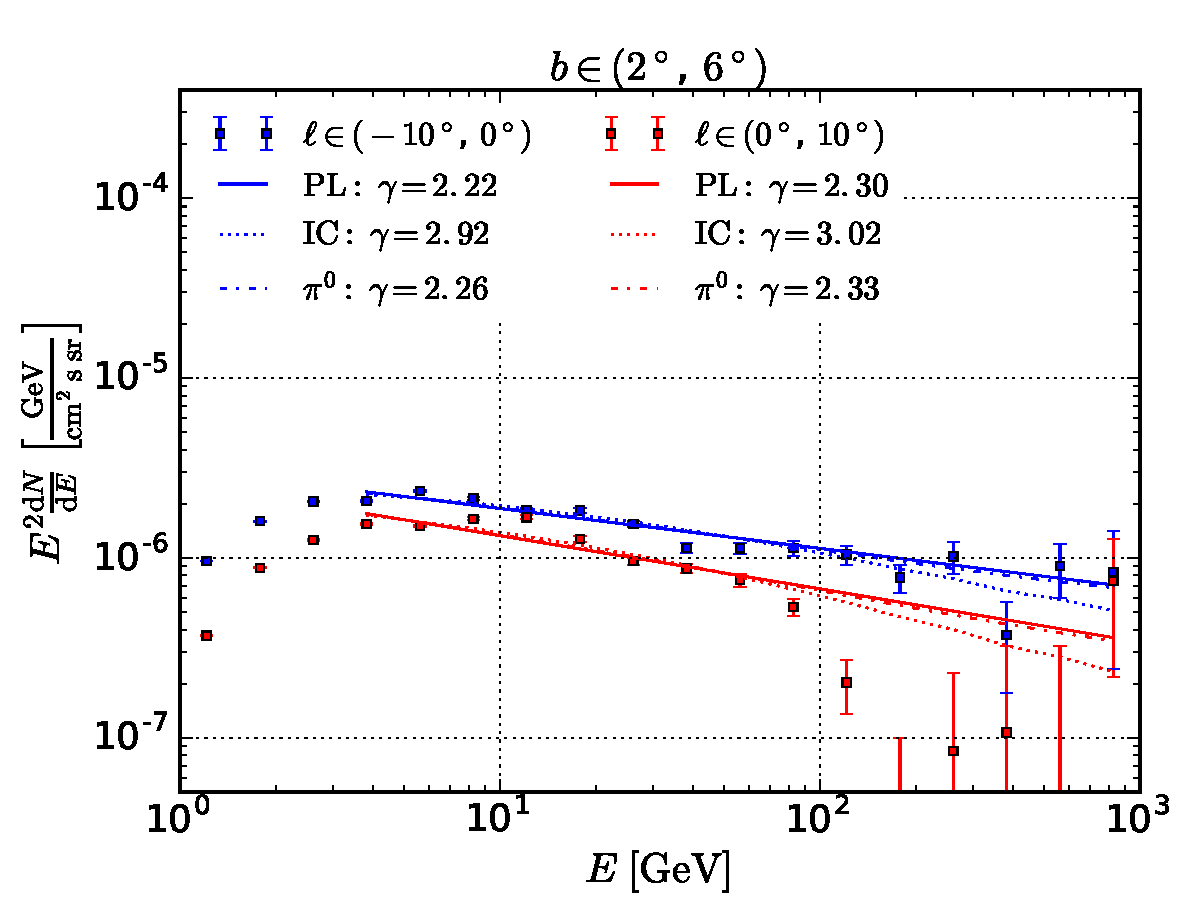
\includegraphics[width=0.5\textwidth]{plots/SED_boxes_source_4.pdf}
%\end{figure}
%\begin{figure}
%	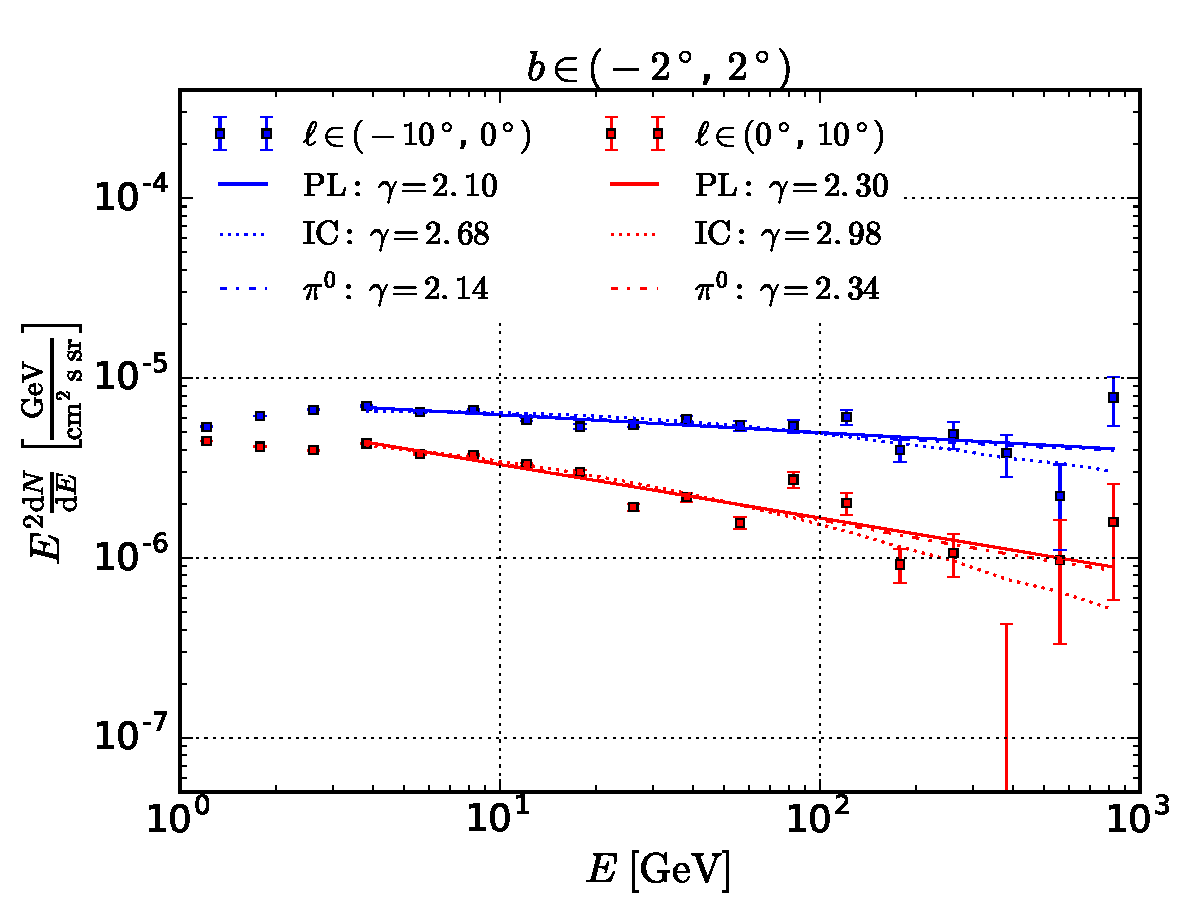
\includegraphics[width=0.5 \textwidth]{plots/SED_boxes_source_0.pdf}
%\end{figure}
%\begin{figure}
%	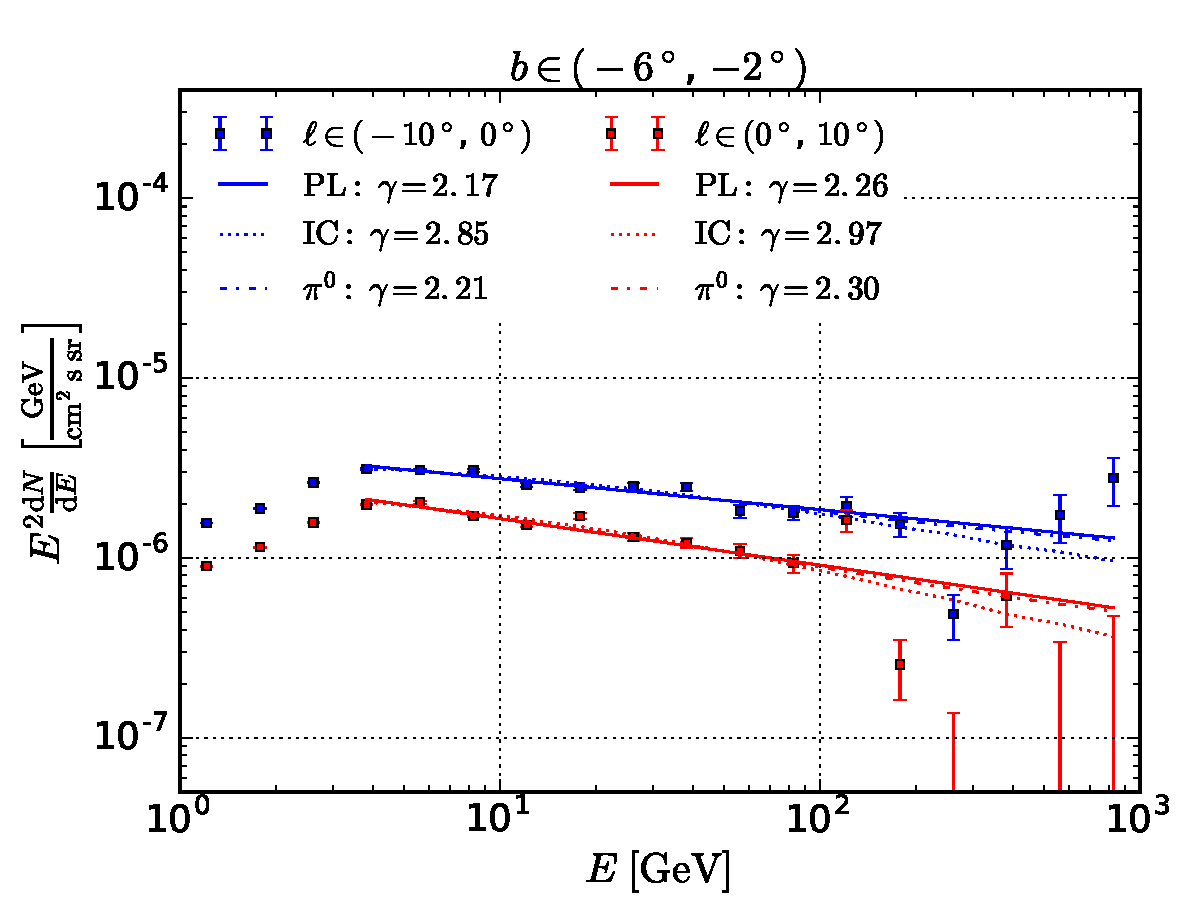
\includegraphics[width=0.5\textwidth]{plots/SED_boxes_source_-4.pdf}
%	\caption{SED of rectangles-model residual in the latitude stripes $(\ang{-2}, \ang{2})$ (left) and $(\ang{-6}, \ang{-2})$ (right) for negative (blue) and positive longitudes (red). We determine the spectral index of a powerlaw (PL), of an electron distribution emitting gamma-rays via IC and of a proton distribution emitting gamma-rays via $\pi^0$-decay.}
%\end{figure}


\subsection{Hadronic model of gamma-ray emission}
\label{sec:Pion_model}

In the hadronic model, the gamma rays are produced as a result of collisions of hadronic CR with the interstellar gas, where $\pi^0$-mesons are created.
The spectrum of the gamma radiation $(E \de n / \de E)_{\gamma,\pi^0}\ [\SI{}{1/cm^3s}]$ depends on the density of interstellar gas, where we assume $n_\Hy = \SI{1}{/cm^3}$, the velocity of CR protons, which we approximate with the speed of light, $v_\pr \approx c$, the (kinetic) energy density of CR protons $(\de n / \de T)_\pr\ [\SI{}{1/GeVcm^3}]$ and the cross section to produce gamma rays in a proton-nucleus collisions $\sigma_\pr (E_\gamma, T_\pr)$, taken from \Laura{reference}:
\be
\left(E\frac{\de n}{\de E}\right)_{\!\!\gamma, \pi^0}\! = \int n_\Hy\ \sigma_\pr v_\pr \left(\frac{\de n}{\de T}\right)_{\!\!\pr} \de T_\pr,
\label{eq:had_spectrum}
\ee
where the integral goes over the kinetic energies of the protons $T_\pr$. Similarly to section \ref{sec:IC_model} we assume for the density of protons a simple powerlaw and determine the normalization $n_\pr$ and spectral index $\gamma_\pr$  by fitting the hadronic spectrum \eqref{eq:had_spectrum} to the diffuse \Fermi data. For that, we again fit the sum of the photon counts generated by hadronic processes and the baseline model for the foreground to the total photon counts detected by the \Fermi-LAT (with PS mask) using Poisson likelihood.  The dotted-dashed line in Figure \ref{fig:SED_with_fits} represents the best-fit hadronic spectrum (labeled as $\pi^0$). The spectral index of the proton spectrum shows a east-west assymmetry. For $b \in (\ang{2}, \ang{6})$ the spectral index to the West of the GC varies between 2.26 and 2.42, for $b \in (-\ang{2}, \ang{2})$ between 2.14 and 2.64 and for $(-\ang{6}, -\ang{2})$ between 2.21 and 2.32. To the East of the GC the indices vary between 2.33 and 3.55. 

We again estimate the probability for the proton spectrum to have an exponential cutoff: For the latitude stripe covering the Galactic plane, $b \in (-\ang{2}, \ang{2})$, adding a cutoff does neither improve the $\chi^2$-valueat negative ($\chi^2 \approx 62$) nor positive longitudes ($\chi^2 \approx 116$). At a $95\%$-confidence level, the lower bound for the cutoff energy for the baseline model (and all models) is $\SI{28.6}{TeV}$ ($\SI{22.6}{TeV}$) for negative longitudes and $\SI{1.8}{TeV}$ ($\SI{11.5}{GeV}$) for positive longitudes.\\
In the latitude band $(-\ang{6}, -\ang{2})$, the $\chi^2$-value does increase both for negative ($\chi^2 = 157$ to $\chi^2 = 123$) and positive longitudes ($\chi^2 = 245$ to $\chi^2 = 156$) by adding an exponential cutoff. The lower bound on the cutoff energy is $\SI{23.6}{TeV}$ ($\SI{0.99}{TeV}$) for negative and $\SI{1.57}{TeV}$ ($\SI{40}{GeV}$) for positive longitudes.

\begin{table*}
  \begin{center}
    \caption{$\chi^2$-values for hadronic-spectrum fit of a distribution of protons following a simple powerlaw and a powerlaw with a cutoff, respectively in the latitude bands discussed in the text. The lower bound for $E_\cut$ at a $\SI{95}{\percent}$-confidence level for our baseline model is shown in the last column; the value in parenthesis gives the lowest value for all models.}
    \label{tab:IC}
    \begin{tabular}{|c|c|c|c|c|} % <-- Alignments: 1st column left, 2nd middle and 3rd right, with vertical lines in between
     	\hline
		 lat & lon  & $\chi^2$(no cutoff) &  $\chi^2$(cutoff) & Lower bound $E_\cut$ \\ 
		\hline
  		$(\ang{2}, \ang{6})$ & east & 416.6 & 70.3 & $\SI{160.6}{GeV}$ ($\SI{160.6}{GeV}$)\\ 
		& west &  127.3 & 204.2 & $\SI{6.3}{TeV}$ ($\SI{1.7}{TeV}$)\\ 
 		\hline
  		$(\ang{-2}, \ang{2})$ & east & 116.4 & 115.5 & $\SI{1.8}{TeV}$ ($\SI{11.5}{GeV}$)\\ 
		& west & 61.5 & 61.5 & $\SI{28.6}{TeV}$ ($\SI{22.6}{TeV}$)\\ 
 		\hline
  		$(\ang{-6}, \ang{-2})$ & east & 127.3 & 83.7 & $\SI{1.57}{TeV}$ ($\SI{40}{GeV}$)\\ 
		& west & 96.7 & 65.0 & $\SI{23.6}{TeV}$ ($\SI{0.99}{TeV}$)\\ 
 \hline
    \end{tabular}
  \end{center}
\end{table*}


\subsection{Summary of the spectral analysis}
%\dima{we can put a summary plot with the baseline model and the band of all spectra in a small subsection here}

\begin{figure}[h]
 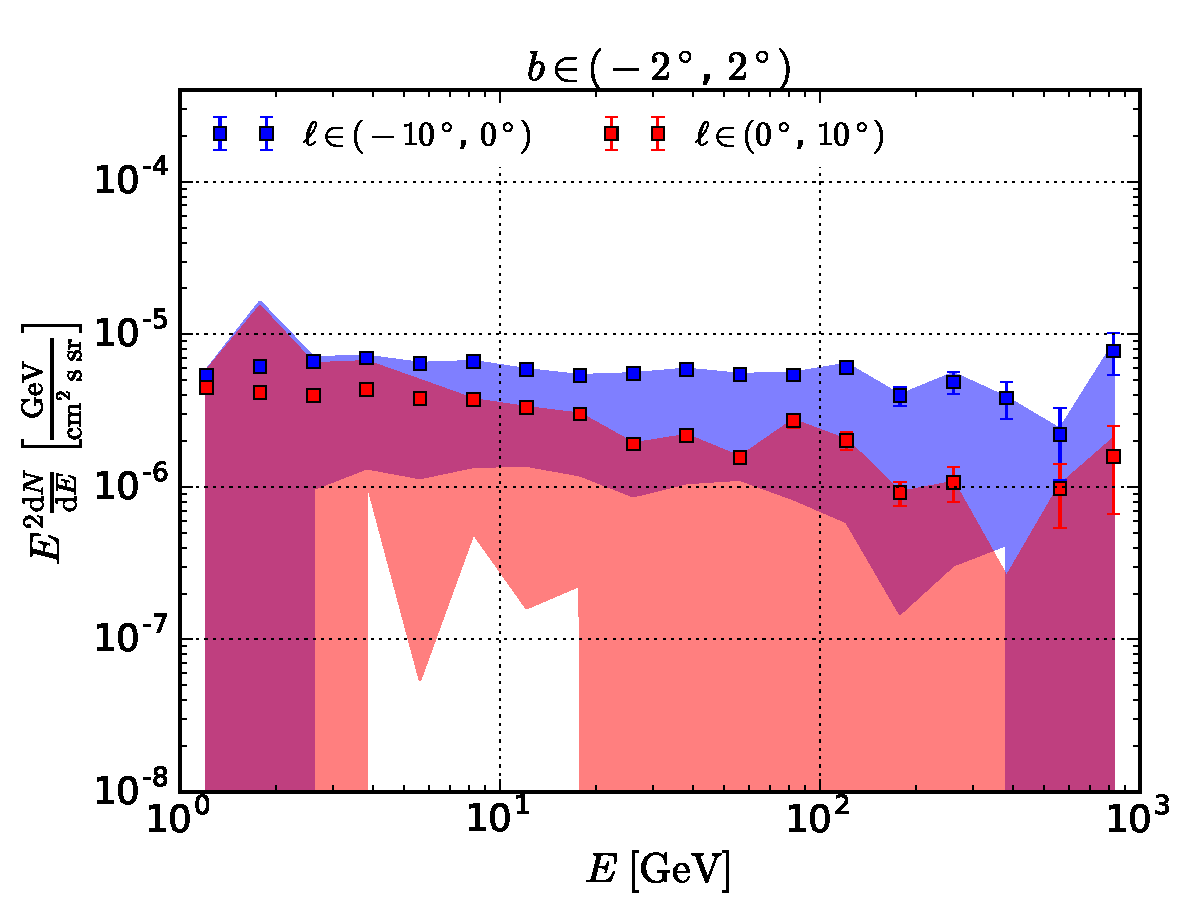
\includegraphics[width=0.5\textwidth]{plots/Summary_SED_0.pdf}
 \caption{SED in the Galactic plane. The shaded areas give the systematic uncertainties estimated from the variation of the other models (using 4 different low-energy ranges).}
 \label{fig:data_diff}
\end{figure}